\chapter[Databáze 2]{B4M36DS2 \\[1ex]\Large{Pojem Big Data, základní principy distribuovaného zpracování dat, typy a vlastnosti NoSQL databází}}
Big Data is high volume, high velocity, and/or high variety information assets that require new forms of processing to enable enhanced decision making, insight discovery and process opimization.

Main characteristics:
\begin{itemize}
    \item Volume (Scale)
    \item Variety (Complexity)
    \item Velocity (Speed)
    \item Veracity (Uncertainty)
\end{itemize}

Additional characteristics:

\begin{itemize}
    \item Value
    \item Value
    \item Validity
    \item Volatility (Period of time the data is valid and should be maintained)
    \item Cardinality
    \item Continuity
    \item Complexity
\end{itemize}


\begin{figure}[ht!]
\centering
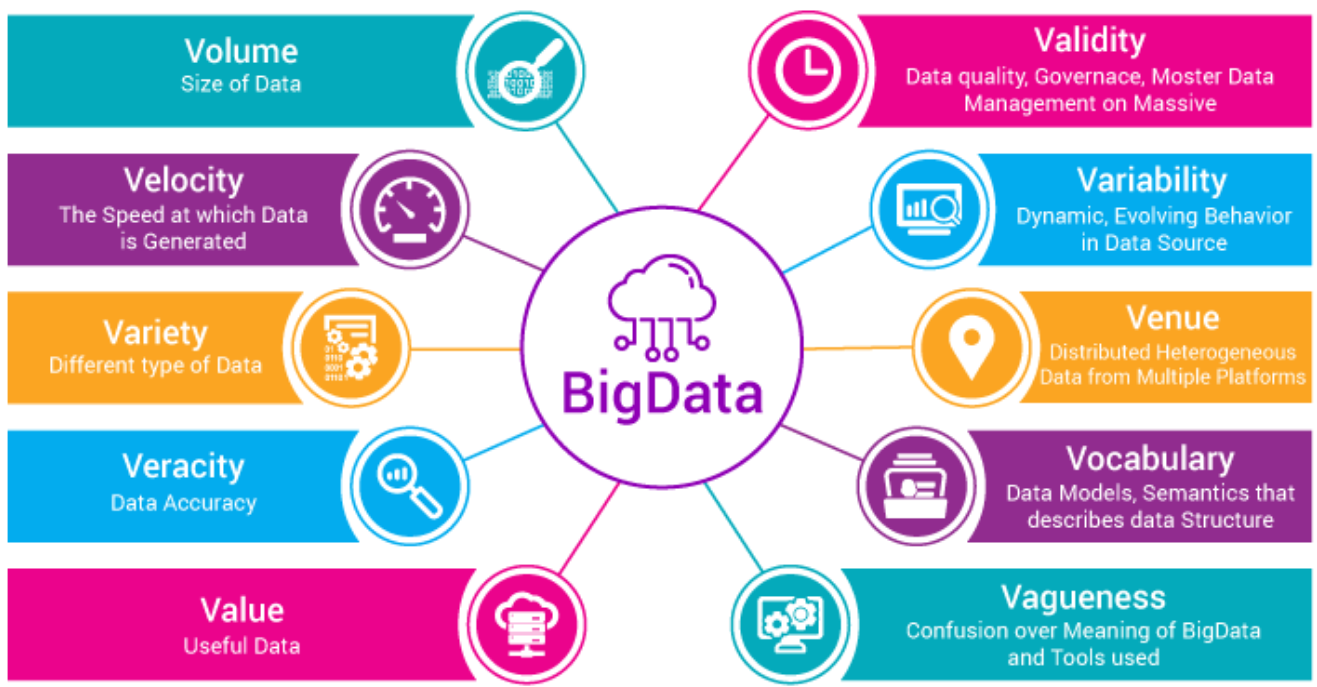
\includegraphics[width=0.8\textwidth]{oborove/DS2/img/bigdata.png}
\end{figure}

\section{Relational DB}
SQL, Normal forms, Selection based on complex conditions, projection, joins, aggregation...
Diminish data redundancy, prevent update anomalies X Data is scattered into small pieces, have to be joined back together when querying

ACID:
\begin{itemize}
    \item \textbf{Atomicity} – partial execution is not allowed (all or nothing)
    \item \textbf{Consistency} – transactions turn one valid database state into another
    \item \textbf{Isolation} – uncommitted effects are concealed among transactions
    \item \textbf{Durability} – effects of committed transactions are permanent
\end{itemize}

Current trends: Distributed file systems, MapReduce and other programming models, cloud computing, NoSQL databases...

\section{NOSQL DB}

\begin{itemize}
    \item KeyValue stores (Redis)
    \item Document stores (Mongo)
    \item Wide Column stores (Cassandra)
    \item Graph Databases (Neo4j)
    \item Native XML Databases (rdf4j) - SPARQL query lang
\end{itemize}

Goal: Respect real world structure of data

\subsection{Aggregate structure}
Data unit with a complex structure. Collection of related data pieces we wish to treat as a unit

Examples:
\begin{itemize}
    \item Value part of key-value pairs in key-value stores
    \item Document in document stores
    \item Row of a column family in wide column stores
\end{itemize}

Types of systems:
\begin{itemize}
    \item Aggregate-ignorant - relational, graph
    \item Aggregate-oriented - key-value, document, wide column
\end{itemize}

No universal strategy how to draw aggregate boundaries. Atomicity: just a single aggregate at a time.

\subsection{Key features}
Elastic scaling - allow scaling horizontally - sharding (splitting) \& replication. Automatic recovery, distribution, tuning. Relaxed (eventual) consistency - BASE instead of ACID:
\newline\newline
BASE:
\begin{itemize}
    \item \textbf{B}asically \textbf{A}vailable - The system works basically all the time, partial failures may occur
    \item \textbf{S}oft State - The system is in flux (unstable), non-deterministic state
    \item \textbf{E}ventual Consistency
\end{itemize}


Advantages:
\begin{itemize}
    \item Scaling - horizontal
    \item Volume - High volumes of data that cannot be handled by RDBMS
    \item Administrators - No longer needed because of the automated maintenance
    \item Economics - Usage of cheap commodity servers
    \item Flexibility - Relaxed or missing data schema, easier design changes
\end{itemize}


Challenges:
\begin{itemize}
    \item Maturity - Often still in pre-production phase with key features missing
    \item Support - Mostly open source, limited sources of credibility
    \item Administration - Sometimes relatively difficult to install and maintain
    \item Analytics  - Missing support for business intelligence and ad-hoc querying
    \item Expertise - Still low number of NoSQL experts available in the market
\end{itemize}

\section{Formats}
\begin{itemize}
    \item XML – Extensible Markup Language
    \item JSON – JavaScript Object Notation
    \item BSON – Binary JSON
    \item RDF – Resource Description Framework
    \begin{itemize}
        \item Subject - Describes a resource the given statement is about
        \item Predicate - Describes the property or characteristic of the subject
        \item Object - Describes the value of that property
    \end{itemize}
    \item CSV – Comma-Separated Values
    \item Protocol Buffers - see ESW
\end{itemize}

\subsection{RDF}

IRI = Internationalized Resource Identifier - URLs are oŌen used in practice

Notations:
\begin{itemize}
    \item N-Triples
    \item Turtle
    \item RDF/XML
\end{itemize}

\subsubsection{N-Triples}
.rdf, Statements are terminated by dots, delimited by EOL, Individual triple components are delimited by spaces, IRIs are enclosed in angle brackets

\begin{figure}[ht!]
\centering
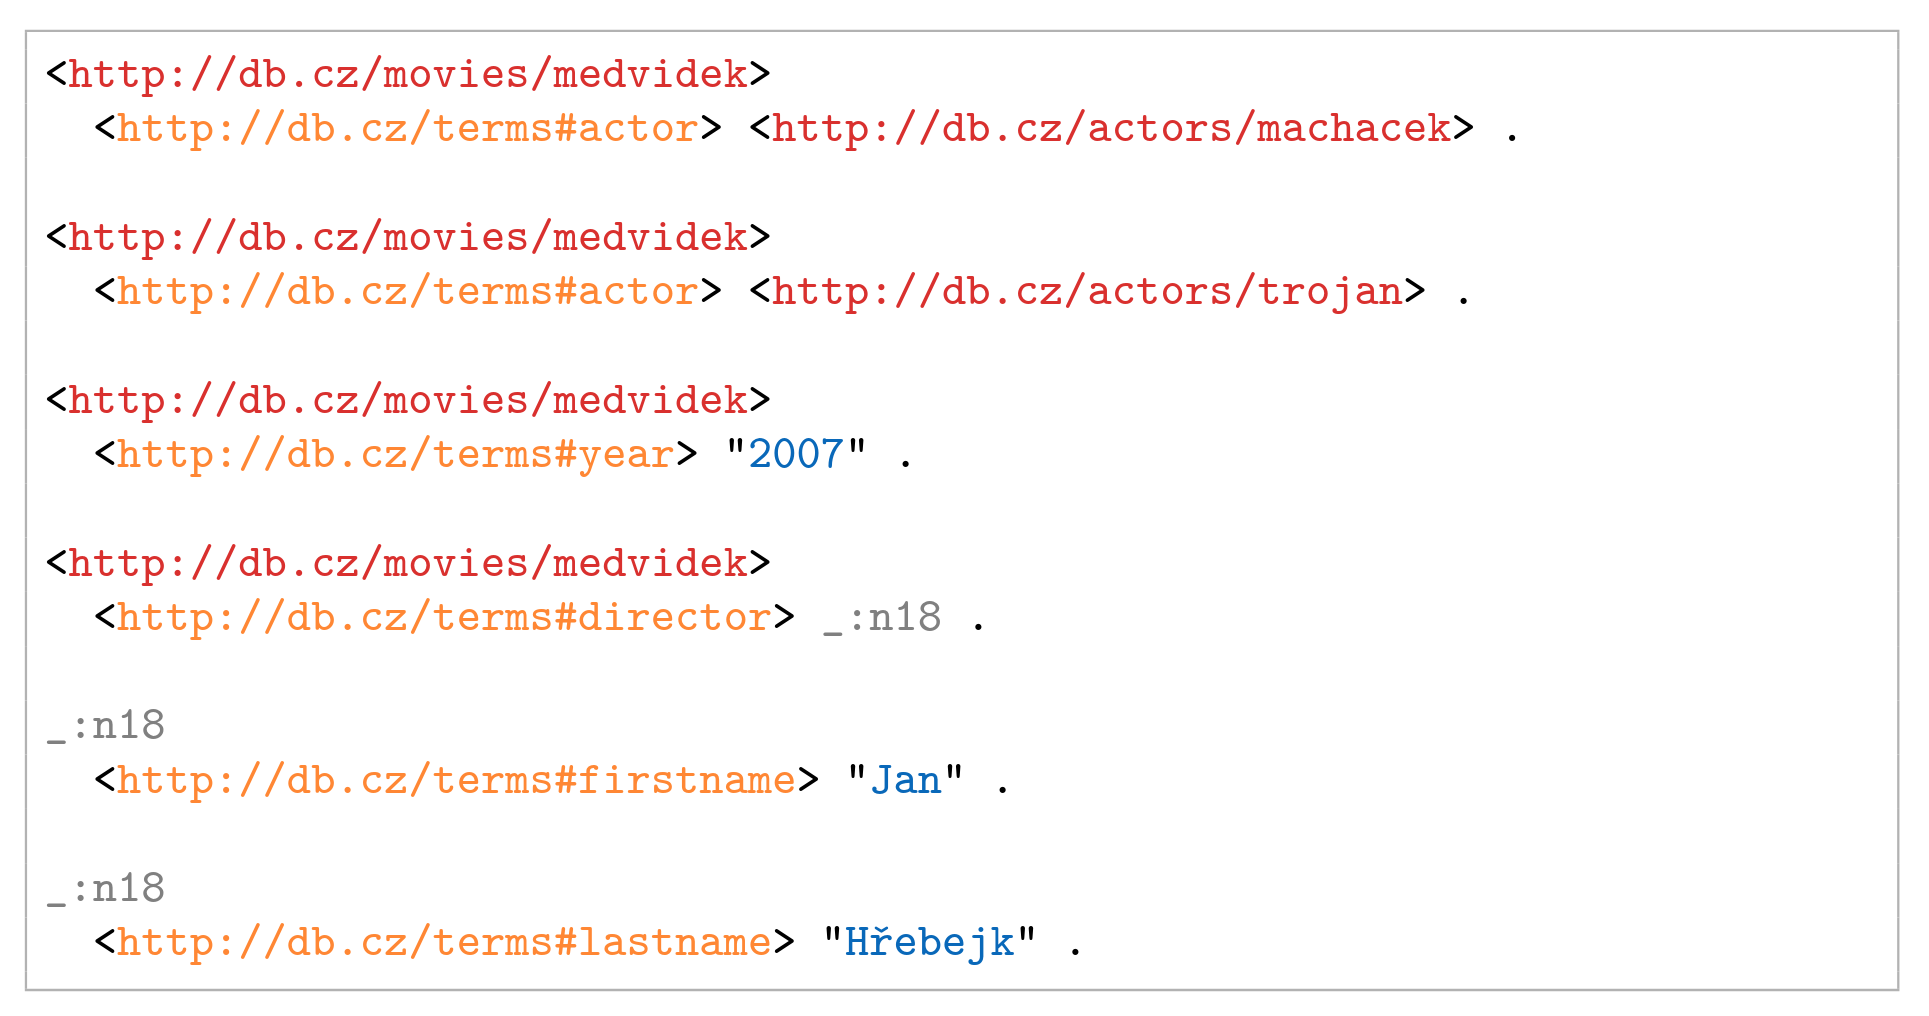
\includegraphics[width=0.8\textwidth]{oborove/DS2/img/ntrip.png}
\end{figure}

\pagebreak
\subsubsection{Turtle}
.ttl, Compact text format, various abbreviations for common usage patterns, sequence of triples and/or declarations. Triples sharing the same subject and object or at least the same subject can be grouped together. Object list for a shared subject and predicate, predicate-object list for a shared subject.

\begin{figure}[ht!]
\centering
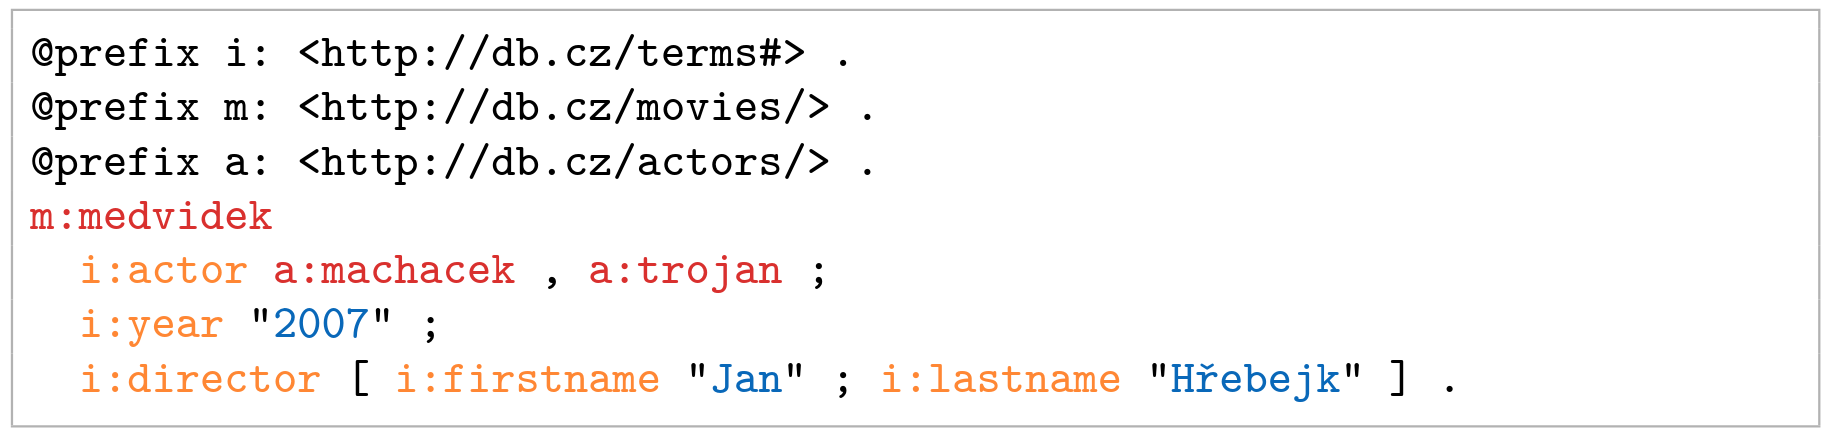
\includegraphics[width=0.8\textwidth]{oborove/DS2/img/turtl.png}
\end{figure}

\section{XQuery}
\begin{figure}[ht!]
\centering
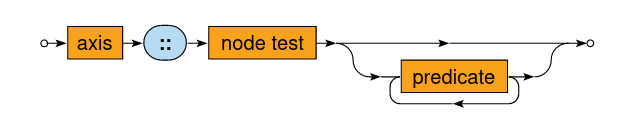
\includegraphics[width=0.5\textwidth]{oborove/DS2/img/xquery.png}
\end{figure}

\textbf{Axis} specifies the relation of nodes to be selected for a given node
\begin{itemize}
    \item Forward axes - self, child, descendant(-or-self), following(-sibling) - The order of the nodes corresponds to the document order
    \item Reverse axes - parent, ancestor(-or-self), preceding(-sibling) - reversed order
    \item Attribute axis – the only axis that selects attributes
\end{itemize}
\textbf{Node tests}
\begin{itemize}
    \item \textbf{name} – all elements / attributes with a given name
    \item \textbf{*} – all elements / attributes
    \item \textbf{node()}– all nodes (i.e. no filtering takes place)
    \item \textbf{text()} – all text nodes
\end{itemize}

\textbf{Predicates}
\begin{figure}[ht!]
\centering
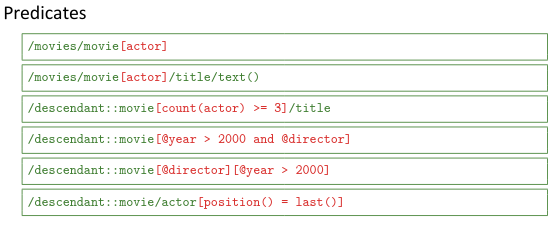
\includegraphics[width=0.55\textwidth]{oborove/DS2/img/pred.png}
\end{figure}

\textbf{Constructors}

Direct - <movies>{ count(//movie) }</movies>

Computed - element movies { count(//movie) }

\begin{figure}[ht!]
\centering
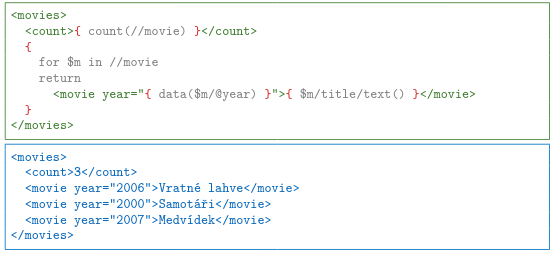
\includegraphics[width=0.55\textwidth]{oborove/DS2/img/direct.png}
\end{figure}
\begin{figure}[ht!]
\centering
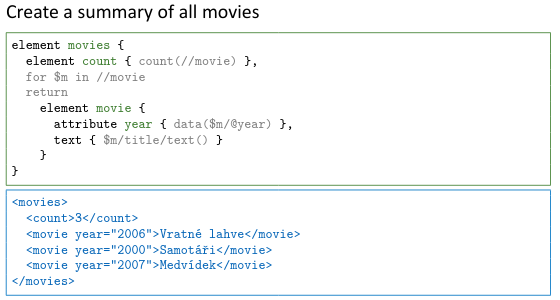
\includegraphics[width=0.55\textwidth]{oborove/DS2/img/computed.png}
\end{figure}

\pagebreak

FLWOR - Versatile construct allowing for iterations over sequences
\begin{figure}[ht!]
\centering
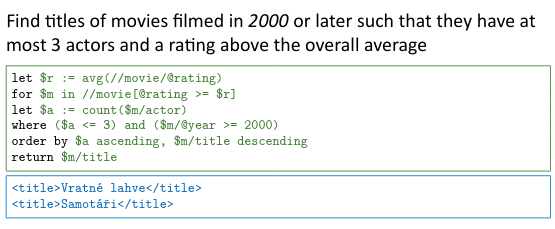
\includegraphics[width=0.75\textwidth]{oborove/DS2/img/flwor.png}
\end{figure}

\section{RDF}
Linked data - SPARQL query lang - Graph patterns, optional graph patterns, subqueries, negation, aggregation, value constructors
\begin{figure}[ht!]
\centering
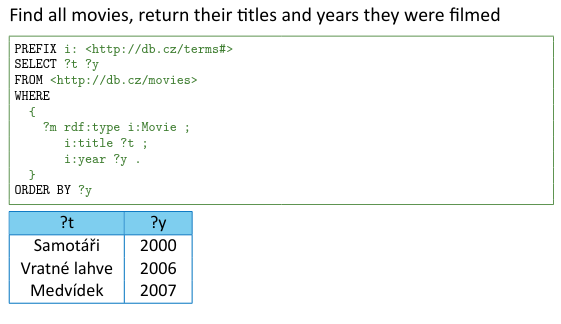
\includegraphics[width=0.75\textwidth]{oborove/DS2/img/sparql.png}
\end{figure}

\section{Map Reduce}
Apache Hadoop - HDFS distributed file system

\begin{itemize}
    \item Map function
    \begin{itemize}
        \item Breaks down a problem into sub-problems
        \item Processes input data in order to generate a set of intermediate key-value pairs
    \end{itemize}
    \item  Reduce function
    \begin{itemize}
        \item Receives and combines sub-solutions to solve the problem
        \item Processes and possibly reduces intermediate values associated with the same intermediate key
    \end{itemize}
\end{itemize}

\begin{figure}[ht!]
\centering
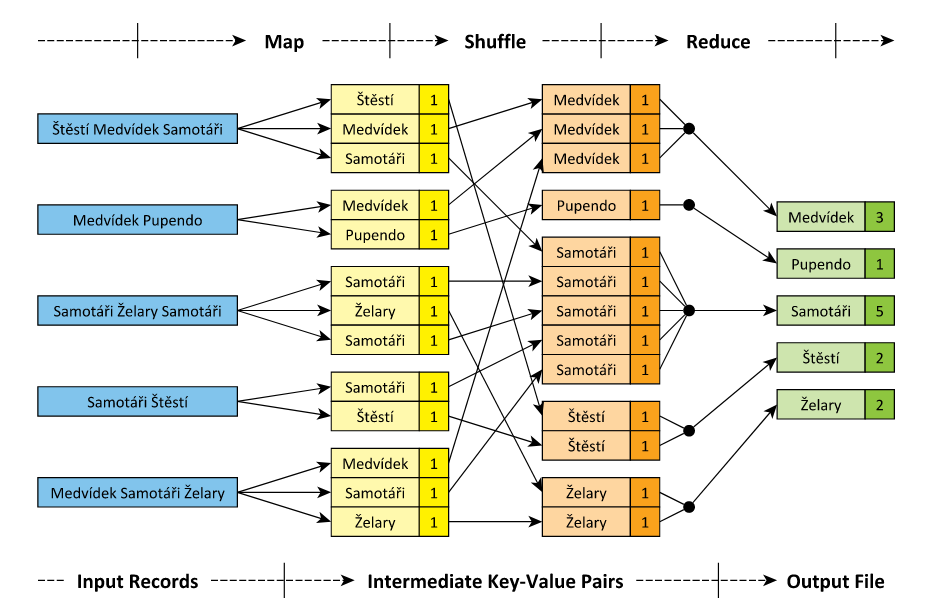
\includegraphics[width=0.75\textwidth]{oborove/DS2/img/mapreduce.png}
\end{figure}

Master - master decides who executes the job, Maintains metadata about input / output files

Slave - Physically store the actual data contents of files, execute jobs

Different slaves run the map and reduce phases, reducers request data from mappers, then send the reduced output to master.

Combine function - Decrease the amount of intermediate data, reduce must be Commutative, Associative and Idempotent

\subsection{Advanced aspects}
Counters: Can be predefined (number of launched/finished Map/Reduce tasks) or custom
Fault tolerance is neccessary:

Worker failure - Master periodically pings every worker, if failed, all its tasks are reset back to their initial idle state and are scheduled on other workers

Master failure

A) periodic checkpoints are created; if master fails, a new copy can then be started

B) master failure is considered to be highly unlikely; users simply resubmit unsuccessful jobs


Stragglers: node that takes unusually long time to complete a task it was assigned. When a MapReduce job is close to completion, the master schedules backup executions of the remaining in-progress tasks. Complete if primary or backup task finishes.

Task granularity: 

Google: 

Map tasks: 16 – 64 MB of input data

Reduce tasks: Small multiple of the number of worker nodes we expect to use

\section{BASIC}
Vertical scaling - scaling server up/down, easy to implement but limits + higher cost + downtime!

Horizontal scaling - across multiple servers, cost effective but data distribution, synchronization, consistency, recovery and latency!

Sharding - Splitting data across nodes - trying to achieve uniform distribution, balanced workload, respect physical location.
These goals may be contradicting/change. Each shard is responsible for storing certain data - Hash partitioning, range partitioning. Problems determining where to read/write. Nodes may contain incomplete/outdated data, nodes or network may fail.

Replication - Same data on different nodes - Master/Slave or Peer to Peer

Master/Slave - Write handled by Master, then propagated to slaves. Read handled by both - Inconsistend read might happen until all slaves synchronized. In case of failure, new Master appointed. Master might be bottleneck.

Peer to peer - more consistency issues - every node can read/write. Synchronization required to avoid conflicts. No bottlenecks.

\subsection{CAP Theorem}
Consistency, Availability, and Partition tolerance

It is not possible to have a distributed system that would guarantee consistency, availability, and partition tolerance at the same time. Only 2 of these 3 properties can be enforced.

Read and write operations must be executed atomically - after a write operation, all readers see the same data

Availability - If a node is working, it must respond to user requests

Partition tolerance - System continues to operate even when two or more sets of nodes get isolated


\textbf{If at most two properties can be guaranteed...}
\begin{itemize}
    \item CA = consistency + availability - Traditional ACID properties - consistency over availability
    \item CP = consistency + partition tolerance - distributed locking
    \item AP = availability + partition tolerance - BASE properties - Cassandra - availability over consistency - Allows levels of scalability that cannot be acquired with ACID
\end{itemize}

\textbf{Consistency} is the lack of contradiction

Write consistency - write-write conflict - Preventing conflicts from occurring (Write locks) X Conflicts may occur, but are detected and resolved later on (Version stamps, vector clocks)

Read consistency - read-write conflict - Propagation of changes to all the replicas takes some time, even the initiator of the write request may read wrong data - Session consistency / read-your-writes / sticky session.


Strong consistency - achievable even in clusters, eventual consistency might often be sufficient

Write quorum: $W > N/2$ - only one write request can get the majority

W = number of nodes successfully participating in the write

N = number of nodes involved in replication (replication factor)

Read quorum: $R >N - W$ - concurrent write requests cannot happen - the newest version is resolved and then returned

R = number of nodes participating in the read


$W = 3$ and read quorum $R = 1$ - All the replicas are always updated

$W = 2$ and read quorum $R = 2$ - Typical configuration, reasonable trade-off


When a quorum is not attained → the request cannot be handled. Quora can be configured to balance read and write workload - The higher the write quorum is required, the lower the read quorum can then be required

\section{Key value stores}
RiakKV - HTTP interface, buckets with objects of a single entity type or objects of various entity types.

Keys - Real-world identifiers (email) or Automatically generated values (autoincrement ID) / Complex keys  (cluster + timestamp)

\begin{figure}[ht!]
\centering
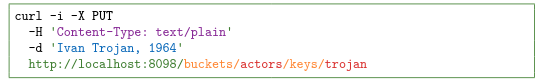
\includegraphics[width=0.75\textwidth]{oborove/DS2/img/riak.png}
\end{figure}


Causal Context - auxiliary data and mechanisms that are necessary in order to resolve the conflicts - Timestamps, vectors clocks, dotted version vectors

Vector clocks - Logical time - Each node has its own logical clock, Initially equal to 0, Incremented by 1 whenever any event takes place, Whenever a message is sent, the local vector is sent as well

\begin{figure}[ht!]
\centering
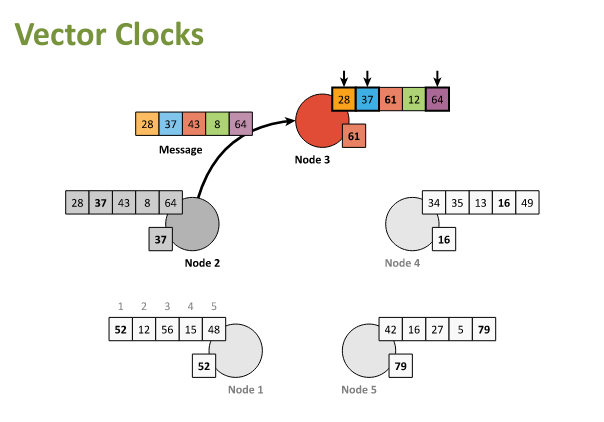
\includegraphics[width=0.75\textwidth]{oborove/DS2/img/vector_clock.png}
\end{figure}


\section{Wide column store}
Uses tables, rows, and columns, but unlike a relational database, the names and format of the columns can vary from row to row in the same table. Column
Column consists of a column name and column value (and possibly other metadata records). Scalar values, but also flat sets, lists or maps may be allowed.

\section{Graph Databases}
Data: a set of entities and their relationships, Basic operations: finding the neighbours of a node, checking if two nodes are connected by an edge, updating the graph structure, ... 

Implementations
\begin{itemize}
    \item \textbf{Adjacency Matrix} - easy to implement but Quadratic space, Addition of nodes is expensive, Retrieval of all the neighbouring nodes takes linear time with respect to
    \item \textbf{Adjacency List} - Needs to checki if there is an edge between two nodes but quick and cheap and compact implementation
    \item \textbf{Incidence Matrix} - good for hypergraphs but requires n x m bits
    \item \textbf{Laplacian Matrix}
    \begin{itemize}
        \item Diagonal of the Laplacian matrix indicates the degree of the node
        \item The rest of positions are set to -1 if the two vertices are connected, 0 otherwise
        \item Allows analyzing the graph structure by means of spectral analysis
    \end{itemize}
\end{itemize}

Improving spatial locality - in graph adjacency matrix representation, exchange rows and columns to improve the cache hit ratio

Bandwidth of a row in a matrix = the maximum distance between nonzero elements, with the condition that one is on the left of the diagonal and the other on the right of the diagonal

Bandwidth of a matrix = maximum of the bandwidth of its rows

Matrices with low bandwidths are more cache friendly - Bandwidth minimization problem (BMP) is NP hard

Graph partitioning - see PAG

Single-relational graphs - Edges are homogeneous in meaning

Multi-relational (property) graphs - Edges are typed or labeled

Types of graph databases: Non-transactional = few numbers of very large graphs; Transactional = large set of small graphs 

Sub-graph queries - Searches for a specific pattern

Super-graph queries - Searches for the graph database members of which their whole structures are contained in the input query

Similarity (approximate matching) queries - Finds graphs which are similar, but not necessarily isomorphic to a given query graph. Key question: how to measure the similarity?

\textbf{Sub-graph queries:}

Mining-Based Graph Indexing Techniques - Effectiveness depends on the quality of mining techniques, Quality of the selected features may degrade over time

Non Mining-Based Indexing Techniques - Can be less effective in their pruning, may need to conduct expensive structure comparisons but can handle graph updates with less cost 

\section{Advanced aspects}

Managing Transactions - Business (longer - eg. shopping) vs System (short); Business transaction = a series of system transactions  

Optimistic Offline Lock - Client operation re-reads any information that the business transaction relies on and it checks that it has not changed

Pessimistic Offline Lock - Forces a business transaction to acquire a lock on each piece of data before it starts to use it; might cause deadlocks

Coarse-grained Lock - A separate lock for individual objects - We need to find them all in order to lock them  

Implicit Lock - If we don't aquire lock, the whole mechanism becomes useless - automatically lock!

Performance tuning - see PAG

Polyglot persistance - we don't care about the underlying database technology, we talk to a service which wraps around the database.
